\documentclass[a4paper]{article}
\usepackage{cmap}
\usepackage{mathtext}
\usepackage{amssymb}
\usepackage{amsmath}
\usepackage[russian]{babel}
\usepackage{indentfirst}
\usepackage[pdftex]{graphicx}
\usepackage{multirow}
\usepackage{mathrsfs}
\usepackage{biblatex}
\usepackage{siunitx}
\usepackage[left=2cm,right=2cm,top=2cm,bottom=2cm]{geometry}
\usepackage{fancyhdr}
\bibliography{bib}
\pagestyle{fancy}
\newcommand{\const}{\mathrm{const}}
\newcommand{\rref}[1]{(\ref{#1})}
\newenvironment{comment}{}{}
\newcommand{\picref}[1]{рис. \ref{#1}}
\newcommand{\mbf}{\mathbf}
\newcommand{\Equip}[3]{
	
	{\bf #1:} $\Delta = \pm #2\; #3$}
\newcommand{\equip}[1]{
	
	{\bf #1}}
\newcommand{\labname}{Дифракция света на ультразвуковой волне в жидкости} 	% название пиши здесь
\newcommand{\labnum}{4.3.2}		% номер вводи здесь
\fancyfoot{}
\fancyhead[RE, RO]{\thepage}
\fancyhead[LE, LO]{Лабораторная работа \labnum \space \labname}
\title{Лабораторная работа \labnum \space \labname} % Название работы здесь
\author{Иван Сладков}
\begin{document}
\maketitle
\thispagestyle{empty}
\section{Аннотация}
В данной работе проводится изучение дифракции света на синусоидальной акустической решётке, а также наблюдение фазовой решётки методом тёмного поля.


\section{Теоретические сведения}

Пусть фаза световых колебаний на передней поверхности жидкости равна нулю. Тогда на задней поверхности (т.е. в плоскости $ z=0 $) она равна \[\varphi = k n L = \varphi_0(1+m \cos \Omega x),\]
где $ L $ -- толщина слоя жидкости в кювете, $ k = 2 \pi /\lambda $ -- волновое число для света, $\lambda $ -- длина световой волны, $ \varphi_0 = k n_0 L $. Таким образом, в плоскости $ z=0 $ фаза световых колебаний является периодической функцией координаты $ x $, иными словами — УЗ-волна в жидкости создаёт фазовую дифракционную решётку.

Её функция пропускания:
\begin{equation}\label{eq:1}
	t(x) = e^{i m \cos \Omega x} \overset{m \ll 1}{\approx} 1 + \frac{im}{2}e^{i \Omega x} + \frac{im}{2}e^{-i \Omega x}.
\end{equation} 
При освещении этой решётки плоской нормально падающей волной амплитуды $ a $ имеем за решёткой (при $ z > 0 $):
\[f(x, z) = a e^{i k z} + \frac{i a m}{2} e^{i(\Omega x +\sqrt{k^2-\Omega^2 } z )}+\frac{i a m}{2} e^{i(-\Omega x +\sqrt{k^2-\Omega^2 } z )}\]
При изучении дифракции методом тёмного поля будем удалять компоненту $ f_0 = a e^{i k z} $ ставя проволочку в соответствующем месте фурье-плоскости. В этом состоит метод тёмного поля в изучении фазово-контрастных объектов. 

При небольших амплитудах звуковой волны показатель преломления жидкости n меняется по закону
\[n=n_0(1+m \cos \Omega x),\]
где $ \Omega $ -- волновое число УЗ волны, $ m\ll 1 $ -- глубина модуляции УЗ волны.

В общем случае после прохождения через кювету световое поле представляет совокупность не трёх, а большого числа плоских волн, распространяющихся под углами, определяемыми условием \begin{equation}\label{eq:лямбдасинустета}
	\Lambda \sin \theta_m = m \lambda, \; m\in \mathbb{Z}.
\end{equation}
Каждая из этих волн соответствует одному из максимумов в дифракционной картине Фраунгофера.
Определяя на опыте положение дифракционных максимумов различного порядка, можно по формуле ()\ref{eq:лямбдасинустета}) найти длину $ \Lambda $ УЗ-волны и вычислить скорость $ v $ распространения ультразвуковых волн в жидкости, если известна частота $ \nu $ колебаний кварцевого излучателя:
\[v = \Lambda \nu .\] 

\section{Оборудование и инструментальные погрешности}

\begin{figure}[tbp]
	\centering
	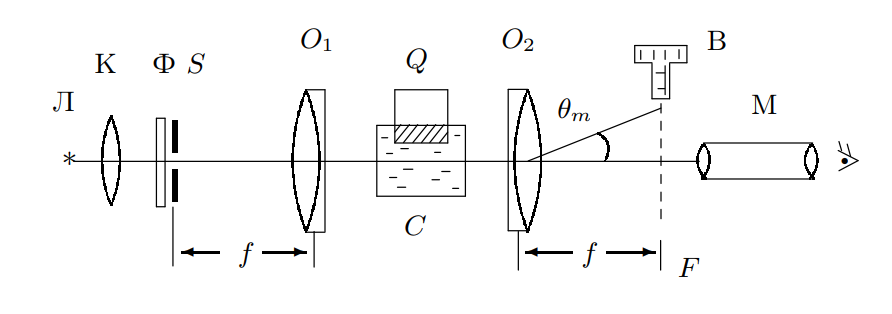
\includegraphics[width=0.8\linewidth]{Screenshot_1}
	\caption{Схема экспериментальной установки}
	\label{fig:screenshot1}
\end{figure}


Схема экспериментальной установки отображена на рис. \ref{fig:screenshot1}.

В работе используются:
\equip{Оптическая скамья}
\equip{Осветитель}: $ \lambda = 6400 \pm 200 \;\SI{}{\angstrom} $
\equip{Длиннофокусные объективы}
\equip{Кювета с жидкостью}
\equip{Кварцевый излучатель с микрометрическим винтом}: $ l = 10 \;мкм/дел $
\Equip{Генератор ультразвуковой частоты}{0.1}{кГц}
\equip{Линза}
\equip{Вертикальная нить на рейтере}
\equip{Микроскоп}

Источник света Л с помощью конденсора К проецируется на входную (коллиматорную) щель S. Входная щель ориентирована горизонтально и прикрыта красным светофильтром Ф. Коллиматорный объектив $ О_1 $ посылает параллельный пучок на кювету с водой C. Излучатель Q, погружённый в кювету, создаёт УЗ-волну. Вертикальное перемещение излучателя осуществляется винтом I, тонкая подача — лимбом II. При определённых положениях излучателя волна становится стоячей.

\section{Результаты измерений и обработка данных}
\emph{Все измерения и расчёты в СИ.}

\paragraph{Исследование по дифракционной картине. }

Оценим \emph{по порядку величины} скорость звука как удвоенное расстояние между наиболее чёткими дифракционными картинами:
\[n = 67 \;дел,\]
\[\lambda \approx 67*10*2=1340 \; мкм. \]
Отсюда 
\[v = \lambda * \nu \approx 1840 \; м/с.\]
Эта величина не является точной, т. к. оценка проводилась по факту наибольшей видимости, поэтому подсчёт погрешностей не имеет смысла.

Определим положения дифракционных полос. Более 5 полос получить не удалось, т. к. генератор имеет низкую чувствительность ручки, а на высоких частотах ($ \gtrsim 5 \; МГц $) выдаёт нестабильную частоту. Результаты в табл. \ref{tab:result}.

% Please add the following required packages to your document preamble:
% \usepackage{multirow}
\begin{table}[h]
	\centering
	\begin{tabular}{|l|l|l|l|l|l|}
		\hline
		\multirow{2}{*}{$\nu, \; МГц$} & \multicolumn{5}{l|}{a, мкм, в порядке n} \\ \cline{2-6} 
		& 0    & +1     & -1      & +2    & -2     \\ \hline
		1.4570                         & 0    & 196    & -172    & 384   & -344   \\ \hline
		2.1515                         & 0    & 272    & -260    & ---   & ---    \\ \hline
		4.3971                         & 0    & 584    & -540    & ---   & ---    \\ \hline
	\end{tabular}
	\caption{Результаты измерений}
	\label{tab:result}
\end{table}

\begin{figure}[tbp]
	\centering
	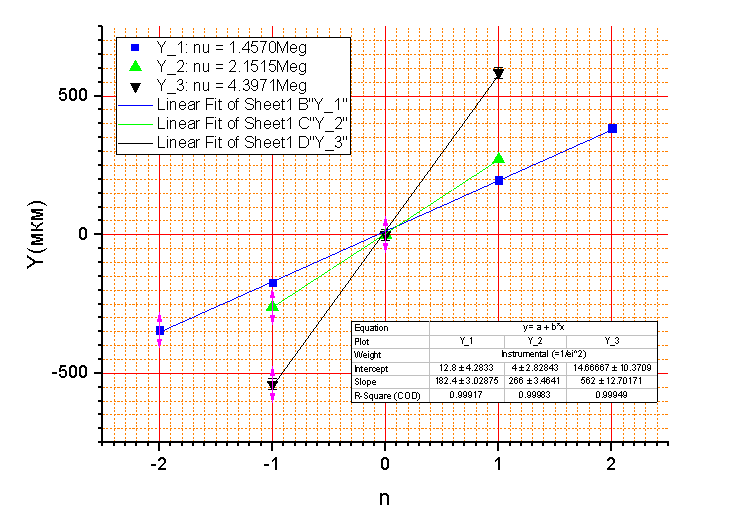
\includegraphics[width=0.8\linewidth]{Screenshot_2}
	\caption{Графики зависимости $Y=Y(n)$}
	\label{fig:2}
\end{figure}


По результатам получим график на рис. \ref{fig:2}. В табл. \ref{tab:2} коэффициенты прямых и полученные по ним результаты из формулы \begin{equation}\label{eq:2}
	v =\nu m f \lambda / l_m = \nu f \lambda / k .
\end{equation} Принимаем во внимание погрешности $ k $, т. к. они существенно больше.


\begin{table}[h]
	\centering
	\begin{tabular}{|l|l|l|l|}
		\hline
		$\nu, \; МГц$ & 1.4570       & 2.1515       & 4.3971       \\ \hline
		$k$           & $182\pm 3$   & $266\pm 4$   & $562\pm 12$  \\ \hline
		$v, \;м/с$    & $1430\pm 20$ & $1450\pm 20$ & $1400\pm 30$ \\ \hline
	\end{tabular}
	\caption{Результат расчёта скорости звука}
	\label{tab:2}
\end{table}

Среднее значение: $$ v = 1430 \pm 50 \; м/с, $$ что близко к табличному значению $ v = 1490  \; м/с $, но не сходится в пределах погрешности. Здесь случайная погрешность среднего взята по формуле среднеквадратичного отклонения (стандартной ошибки) и сложена с инструментальной по формуле $ \sqrt{\sigma^2+\delta^2} $.

\paragraph{Исследование методом тёмного поля. }

Найдём цену деления шкалы микроскопа через период сетки $ h = 1 \;мм $. $ n = 22\; дел/кл $, т. е. $ 1\; дел = 45\; мкм $

По формуле $ \Lambda = 45\;мкм * 2 * n / m $ найдём длину ультразвуковой волны.
Результаты измерений и расчётов в табл. \ref{tab:3}.

\begin{table}[h]
	\centering
	\begin{tabular}{|l|l|l|l|}
		\hline
		$\nu, \; МГц$     & 1.7070 & 2.0866 & 4.2673 \\ \hline
		$n, \; дел$       & 65     & 44     & 43     \\ \hline
		$m, \; линий$     & 8      & 7      & 14     \\ \hline
		$\Lambda, \; мкм$ & 183    & 142    & 69     \\ \hline
	\end{tabular}
	\caption{Результат измерения длин волны}
	\label{tab:3}
\end{table}

\begin{figure}[tbp]
	\centering
	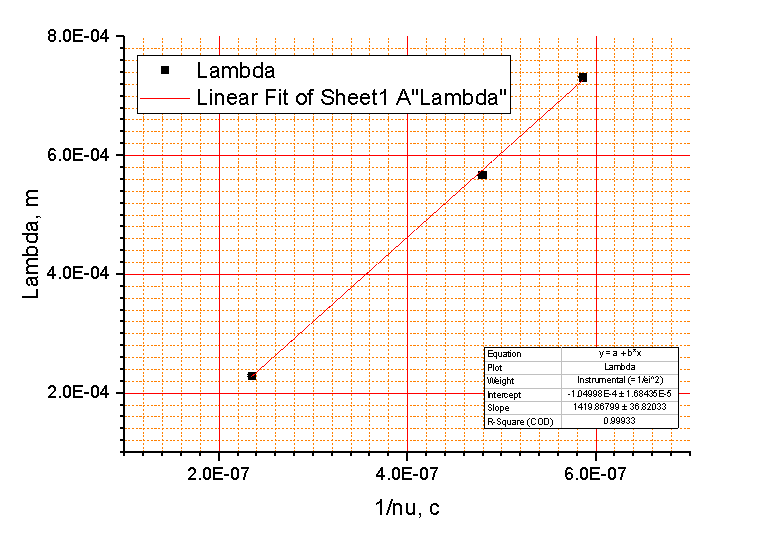
\includegraphics[width=0.8\linewidth]{Screenshot_3}
	\caption{Зависимость $\Lambda = \Lambda (1/\nu)$}
	\label{fig:3}
\end{figure}


Отсюда по графику на рис. \ref{fig:3} найдём скорость звука в жидкости: $$ v = 1419 \pm 40 \; м/с, $$ что согласуется с полученными ранее результатами, но вновь не совпадает с табличными данными. В данном случае учтена погрешность только по МНК, т. к. считаем инструментальные погрешности достаточно низкими.

\paragraph{Качественные наблюдения. } Закрывая ненулевые максимумы получаем равномерную засветку, так как интенсивность нулевого максимума многократно превышает интенсивность ненулевых (связано со свойствами дифракции Фраунгофера).

\section{Вывод}
К сожалению, не удалось провести достаточное количество замеров и получить достаточно чётких полос. В основном это связано с особенностями аппаратуры, применяемой в опыте, в особенности, с глючным генератором частоты. 

Так или иначе, удалось с неплохой точностью измерить скорость звука в воде используя волны сжатие-разряжение как синусоидальную решётку; кроме того, была изучена дифракция света на такой акустической решётке; был применён и изучен метод тёмного поля в наблюдении фазовых объектов.


\begin{thebibliography}{9}
	\bibitem{Siv} Сивухин Д. В. \emph{Общий курс физики. Том 4 Оптика}, 2004
	\bibitem{kir} Кириченко Н. А. \emph{Принципы оптики}, 2014
	\bibitem{max} \emph{Лабораторный практикум по общей физике. В 3 томах. Том 2. Оптика: учебное пособие} под ред. А. В. Максимычева
\end{thebibliography}
\end{document}